\documentclass[10pt,twocolumn,letterpaper]{article}

\usepackage{iccv}
\usepackage{times}
\usepackage{epsfig}
\usepackage{graphicx}
\usepackage{amsmath}
\usepackage{amssymb}
\usepackage{subfigure}
% Include other packages here, before hyperref.
  
% If you comment hyperref and then uncomment it, you should delete
% egpaper.aux before re-running latex.  (Or just hit 'q' on the first latex
% run, let it finish, and you should be clear).
\usepackage[pagebackref=true,breaklinks=true,letterpaper=true,colorlinks,bookmarks=false]{hyperref}

\DeclareMathOperator*{\argmin}{\arg\!\min}
%\DeclareMathOperator*{\simi}{\sim\!}
\iccvfinalcopy % *** Uncomment this line for the final submission

\def\iccvPaperID{183} % *** Enter the ICCV Paper ID here
\def\httilde{\mbox{\tt\raisebox{-.5ex}{\symbol{126}}}}

% Pages are numbered in submission mode, and unnumbered in camera-ready
\ificcvfinal\pagestyle{empty}\fi
\begin{document}

%%%%%%%%% TITLE
%\title{Talk to the Machine: What can we Learn From Natural Language Video Descriptions?}
\title{Video Event Understanding using Natural Language Descriptions}

\author{Vignesh Ramanathan$^*$ \quad \quad Percy Liang$^\dagger$ \quad \quad Li Fei-Fei$^\dagger$ \\
$^*$Department of Electrical Engineering, Stanford University \\
$^\dagger$Computer Science Department, Stanford University\\
{\tt\small \{vigneshr, pliang, feifeili\}@cs.stanford.edu}
}
\maketitle
%\thispagestyle{empty}

%%%%%%%%% ABSTRACT
\begin{abstract}
Human action and role recognition play an important part in complex event understanding. 
State-of-the-art methods learn action and role models from detailed spatio-temporal annotations, 
which requires extensive human effort. 
In this work, we propose a method to learn such models based on natural language descriptions of the training videos, 
which are easier to collect and scale with the number of actions and roles. 
There are two challenges with using this form of weak supervision: First, these descriptions only provide a high-level summary 
and often do not directly mention the actions and roles occurring in a video. 
Second, natural language descriptions do not provide spatio-temporal annotations of actions and roles. 
To tackle these challenges, we introduce a topic-based semantic relatedness (SR) measure between a video description 
and an action and role string, and incorporate it into a posterior regularization objective. 
Our event recognition system based on these action and role models matches the state-of-the-art method on 
the TRECVID-MED11 event kit, despite weaker supervision. %detailed spatio-temporal annotations
\end{abstract}

%%%%%%%%% BODY TEXT
\section{Introduction}
The ability to differentiate complex events is a key step towards video
understanding and has spurred significant research in recent years
\cite{Merler_ITM12, Izadinia_ECCV12, Rohrbach_ECCV12}. Complex
events can be thought of as compositions of atomic actions performed by
people holding different roles. In this work, we provide a method to
learn these action and role models based on easily obtainable natural language
descriptions of event videos (see Fig.~\ref{fig:pull_figure}). We rely
entirely on these descriptions and do not require separate ground truth annotations
of roles and actions.

% -------- System figure
\begin{figure}[ht!]
\centering
   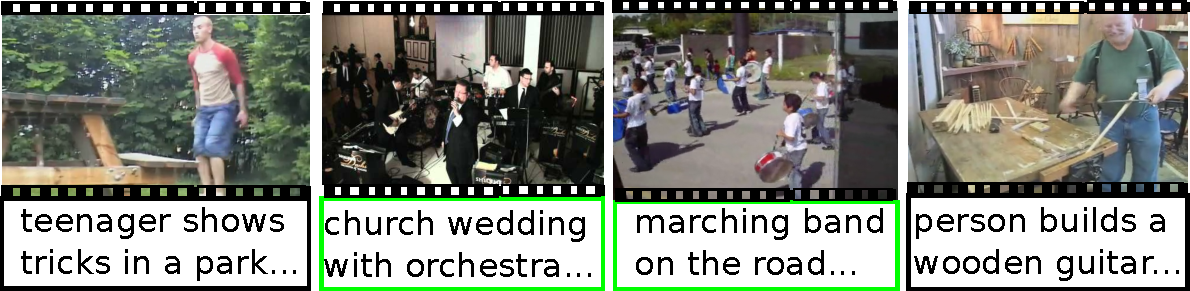
\includegraphics[scale = 0.4]{../images/pullFigure_2.pdf}
      \caption{Our method relies on natural language video descriptions to
      train action and role models. Sample videos along with their
      descriptions are shown.
      The descriptions of videos containing the action
      ``play instrument'' are bounded in green,
      but we do not use action/role labels during training.}
\label{fig:pull_figure}
\end{figure}
% ---------------------------------------------------------------------------------

The use of action and/or role models trained with extensive spatio-temporal
annotations has shown to boost event recognition performance in videos
\cite{Izadinia_ECCV12, Lan_CVPR12}. Such detailed annotations require expensive
human effort and severely restrict the scalability with the inclusion of more
actions and roles.
On the other hand, complex event datasets like TRECVID-MED11 \cite{MED11} event kit and \textit{MPII} Cooking
\cite{Regneri_TACL13} are accompanied by natural language descriptions,
which are easy to obtain and incur only a one-time annotation cost during the
collection of a dataset.
Internet repositories such as YouTube already have accompanying descriptions,
and require no annotation at all.
%they can be gathered from the text
%accompanying the videos in case of Internet datasets.
%We exploit such descriptions completely to learn atomic action and role models.

% First
Unfortunately,
natural language descriptions only provide a \emph{coarse} high-level summary of the events
occurring in videos.
This coarseness leads to two challenges.
First, the canonical action labels (e.g., ``play instrument'')
might not appear in the description (e.g., ``church wedding with orchestra'')---see
Fig.\ref{fig:pull_figure}.
%As demonstrated by the positive training examples of the action
%``play instrument'' in Fig.~\ref{fig:pull_figure}, the video description might
%not contain an action string, but still imply its presence (in this
%case through an ``orchestra'' or a ``marching band'').
Bridging the gap between high-level natural language descriptions and low-level action/role labels
is a challenging problem in natural language semantics.
To tackle this, we define a new semantic
relatedness (SR) measure between an action/role label and a natural language description.
The measure is based on Latent Dirichlet Allocation \cite{???} trained on
YouTube descriptions.
%We construct a language topic model specific to the task and use it to
%define the SR measure.
%We also handle outliers introduced by this measure
%through self-paced learning.

% -------- System figure
\begin{figure*} 
  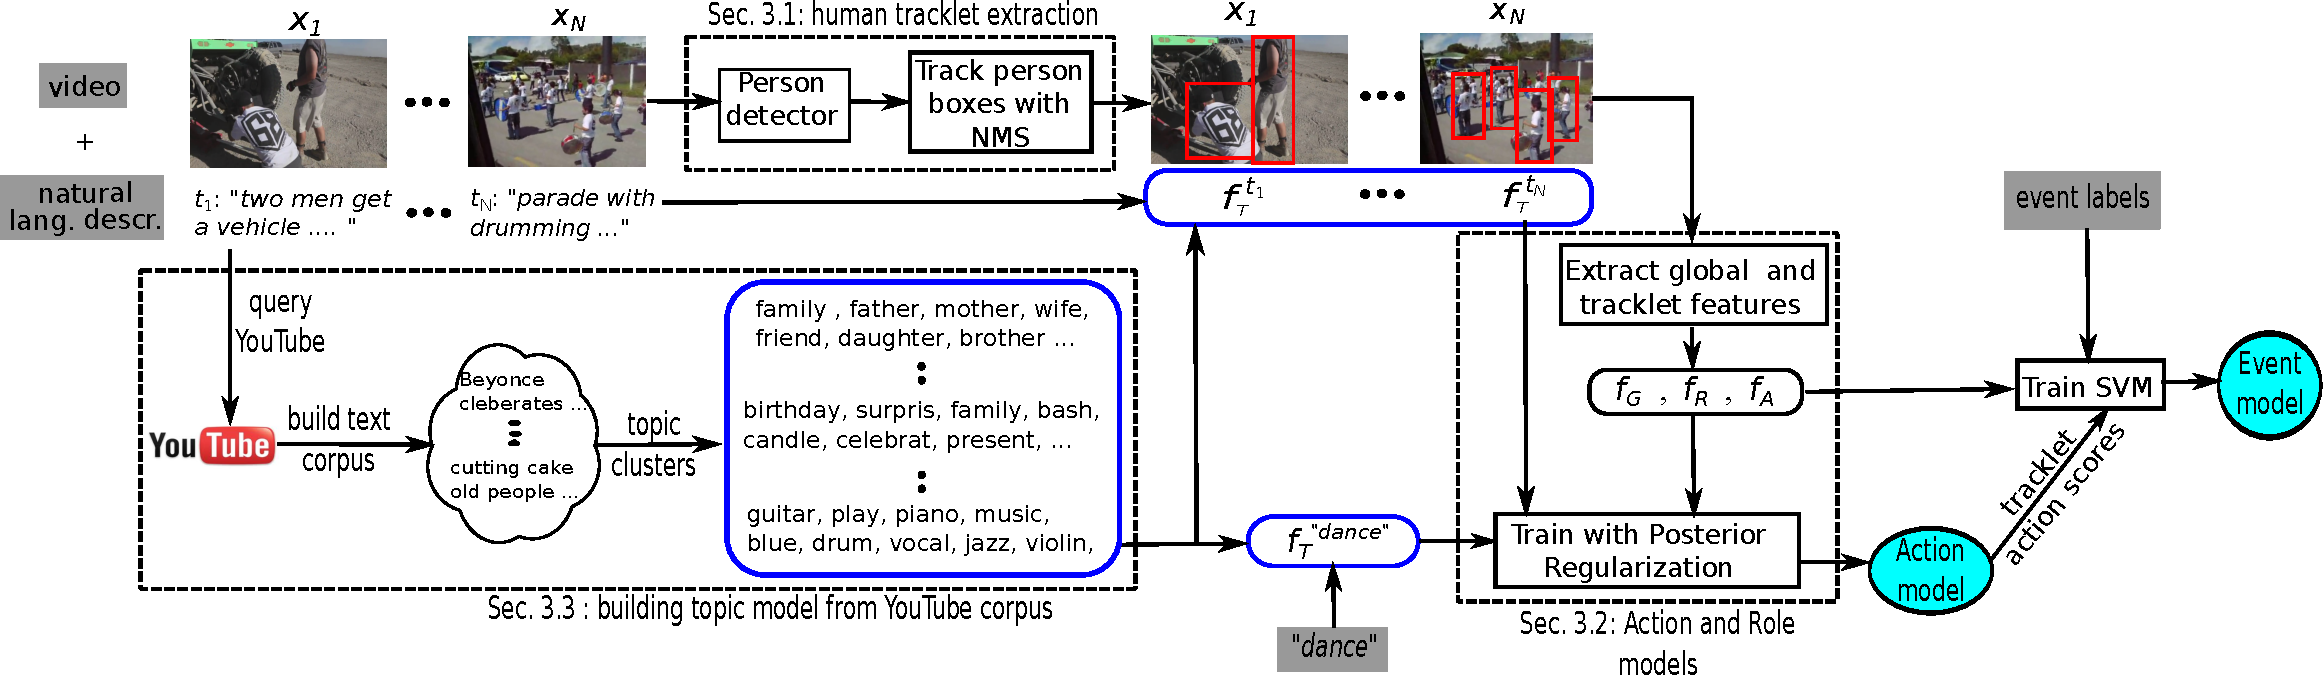
\includegraphics[scale = 0.44]{../images/system_e.pdf}
  \caption{An overview of the system. Inputs to the system are shaded in grey.}
\label{fig:system}
\end{figure*}
% ---------------------------------------------------------------------------------

The second challenge is that natural language descriptions do not specify the
spatiotemporal extents of actions and roles.
To cope with this missing data, we use the Posterior Regularization
(PR) framework \cite{Ganchev_JMLR10}.
Specifically, we represent a video as a
bag of spatiotemporally-localized human tracklets,
and define an action and role assignment variable for each tracklet.
The natural language supervision then imposes a soft constraint
that at least one of tracklets in the video is assigned to a semantically-related action/role label.

%PR allows us to learn enforcing
%constraints regarding the presence or absence of action and role tracklets in
%the training videos. 

We first evaluated our approach on action and role classification,
showing that our SR measure improves accuracy over existing measures.
We also considered event recognition, where the state-of-the-art method \cite{Izadinia_ECCV12} requires
detailed spatiotemporal annotations of atomic actions.
We incorporated our action/role models, which are trained only on natural language descriptions,
into our event recognition model.
On the TRECVID-MED11 event kit,
our model matches \cite{Izadinia_ECCV12} despite using weaker supervision.

%The key contributions of our work can be summarized as follows:
%\vspace*{-5pt}
%\begin{enumerate}
% \item We introduce a framework for using compelte natural language descriptions to learn atomic action and role models, which are used to achieve state-of-the-art event recognition performance on the TRECVID-MED11 event-kits.\vspace*{-5pt}
% \item We present a method to identify the semantic relatedness of a description to an action/role query. We propose a self-paced method which use this measure to identify positive and negative training examples for model learning.\vspace*{-5pt}
% \item We develop a posterior regularized model, which treats a video as a bag of human tracklets for action and role recognition in the absence of temporal annotation.\vspace*{-5pt}
%\end{enumerate}
%\vspace*{-5pt}

\section{Related Work}
\noindent \textbf{Natural language processing for vision} 
Recent works attempting to leverage the vast amount of textual data available with Internet images have 
developed vision-specific semantic relatedness measures \cite{Rohrbach_CVPR10, Rohrbach_ECCV10} 
to identify the link between part-based object attributes and image classes. 
However, such measures are derived from general text like Wikipedia, 
and are therefore, less suited for language pertaining to human actions/roles specific to a set of events. 
Other attempts to use textual descriptions in conjunction with attribute recognition were 
presented in \cite{Berg_ECCV10, Parikh_CVPR11}. 
While, \cite{Berg_ECCV10} is restricted to simple part-based attributes directly mentioned in the image description,
\cite{Parikh_CVPR11} involves humans in the loop to actively describe a group of images through visual attributes. 
Another line of work \cite{Jia_ICCV11, Socher_CVPR10} jointly considers multiple modalities including text descriptions to perform image annotation, retrieval or segmentation. 
\cite{Rohrbach_ECCV12}  transfers composite action videos to an attribute space enabling comparison with textual corpus. % describing activities in terms of these attributes. %While demonstrating a method to use external knowledge from text data, this method still requires video annotations to learn atomic action attribute classifiers. 

Previous works like \cite{Laptev_CVPR08, Marszalek_CVPR09, Cour_ECCV08, Everingham_BMVC06} use 
time-synchronized movie scripts or closed captions to identify video segments corresponding to specific actions. 
Again, these methods rely on presence of the action label in the script or use a pre-trained classifier \cite{Laptev_CVPR08} 
to identify the action-text in a script and require temporal annotations. 
\cite{Yang_CVPR11} performs tag prediction by using meta data provided along with YouTube videos. 
\cite{Motwani_ECAI12} processes descriptions of action segments to automatically discover a set of action classes.

In contrast to the above methods, we learn models based on natural language
descriptions which may not contain the action and role label. In particular, we
construct a topic-model based measure specific to our task.
\\
\noindent \textbf{Action, role and event recognition} \cite{Izadinia_ECCV12,
Lan_CVPR12} showed significant improvement in event recognition by using atomic
action and role detectors as a part of their event recognition model. Both
methods required spatio-temporal annotation of action and roles in the
training videos to learn the models. Other works which have investigated the
use of social roles in video understanding include \cite{Wang_ECCV10, Fathi_CVPR12}. \cite{Liu_CVPR11} uses attributes to perform action
recognition in videos. 
\\
\noindent \textbf{Weakly supervised action models} 
Discriminative spatio-temporal regions in videos or images to localize the actions in \cite{Satkin_ECCV10, Raptis_ECCV12, Singh_ECCV12}.
Similar in spirit to these works, we try to localize the human actions and roles. 
However, we develop a model with latent action and role assignments to different human tracklets in a video.

\section{Our Approach} \label{sec:model_formualation}

An overview of our system is shown in Fig.~\ref{fig:system}. We first use
natural language video descriptions to train action and role models.  The prediction probabilites
from the model are then used to train event recognition models.

In our setup, each training video is accompanied by a natural language
description, which might or might not contain the action label
present in the video.
Formally, we denote our training dataset by
$\left(\langle x_1, t_1 \rangle, \dots , \langle x_n, t_n\rangle \right)$,
where $x_i$ is a video belonging to different event classes and
$t_i$ is the corresponding textual description. 
No textual descriptions are present in the test data.

We assume a fixed set of actions $\mathcal{A}$ and roles $\mathcal{R}$ and define additional variables $\langle y_i, z_i \rangle$ for each $x_i$. 
Here, $y_i^a \in \{-1,0,1\}$ indicates whether the label of the video corresponding
to the action $a$ is negative, unknown or positive. We define $z_i^r \in \{-1,0,1\}$ similarly for the role $r$. 
These variables are not observed in the training data.


\subsection{Human tracklet extraction}
Complex event videos are composed of many atomic actions and roles, 
confined to spatio temporal regions. 
We attempt to incorporate this locality by representing a video as a bag of human tracklets. 
We assume that the action or role occurring in a video would then correspond to one or more of these tracklets. 
As illustrated in the corresponding section of Fig.~\ref{fig:system}, 
we obtain tracklets by running a human detector \cite{Felzenszwalb_PAMI10} across different segments in a video 
and tracking the resulting bounding boxes within a temporal window of $100$ frames. 
In our experiments, we uniformly partition a video into $20$ different segments and obtain $5$ tracklets in each segment 
based on non-maximal suppression. We choose the top $50$ tracklets based on their detection scores.

\subsection{Action and role model}\label{sec:model_features}
We define a conditional random field (CRF) encompassing the action and role relation between different tracklets
in a video similar in spirit to \cite{Lan_CVPR12}. 
However, we do not assume perfect human tracking, 
and complete person-wise action and role labels for training. 

We assume that each video $x_i$ has a set of human tracklets given by $\mathcal{H}_i$. 
The potential $\Phi(x, h, a, r)$ of making
action assignment $a$ and role assignment $r$ to the tracklet $h$ in video $x$ is given in Eq.~\ref{eq:potential_tracklet}.
\vspace{-4pt}
\begin{eqnarray}\label{eq:potential_tracklet}
  \Phi(x, h, a, r) & = & w_{g}(a,r) \cdot f_{g}^x + w_{in.}(a,r) \\ \nonumber
                   & & + w_{ac.}(a) \cdot f_{ac.}^h + w_{ro.}(r) \cdot f_{ro.}^h, \nonumber
\end{eqnarray} where $f_g^x$ is the $d_g$ dimensional global video feature of $x$. The $d_{ac.}$ dimensional feature
$f_{ac.}^h$, and $d_{ro.}$ dimensional feature $f_{ro.}^h$ are the action and role features 
for the human tracklet $h$ respectively. The global weight is denoted 
by $w_g \in \mathbb{R}^{|\mathcal{A}| \times |\mathcal{R}| \times d_g}$, where $w_g(a,r) \in \mathbb{R}^{d_g}$
gives the global weight for action $a$ and role $r$.
Similarly, $w_{in.} \in \mathbb{R}^{|\mathcal{A}| \times |\mathcal{R}|}$ is the weight for joint 
action and role assignment to a track, with $w_{in.}(a,r) \in \mathbb{R}$ corresponding to action $a$ and role $r$. 
The weight $w_{ac.} \in \mathbb{R}^{|\mathcal{A}| \times d_{ac.}}$
is the action-weight and $w_{ro.} \in \mathbb{R}^{|\mathcal{A}| \times d_{ro.}}$ is the role-weight. The action-weight corresponding
to $a$ is given by $w_{ac.}(a) \in \mathbb{R}^{d_{ac.}}$ and the role-weight for role $r$ is given by $w_{ro.}(r) \in \mathbb{R}^{d_{ro.}}$.
The weights to be learned are then represented by $w = (w_g, w_{in.}, w_{ac.}, w_{ro.})$.

With a slight abuse of notation, we let $a_i \in \mathcal{A}^{|\mathcal{H}_i|}$ be the action-labels assigned to the tracks in video $x_i$, 
and $a_i^h \in \mathcal{A}$ denote the action-label of the track $h$ in the video. 
Similarly, we let $r_i \in \mathcal{R}^{|\mathcal{H}_i|}$ be the role-labels associated with $x_i$ and $r_i^h \in \mathcal{R}$ be the role-label of track $h$.
The probability $p(a_i, r_i; w)$ of this assignment to video $x_i$ is given by Eq.~\ref{eq:prob_assignment}.
\vspace{-4pt}
\begin{eqnarray}\label{eq:prob_assignment}
  p(a_i, r_i; w) = \frac{1}{Z_i} \exp \left(\sum \limits_{h \in \mathcal{H}_i} \Phi(x_i, h, a_i^h, r_i^h) \right),
\end{eqnarray}, where $Z_i$ is the partition function for the video $x_i$.

The log-likelihood of making action and role assignments $\mathbf{a}, \mathbf{r}$ respectively across all videos is
given by Eq.~\ref{eq:log_likelihood}

\begin{eqnarray}\label{eq:log_likelihood}
  L(\mathbf{a}, \mathbf{r}; w) = \sum \limits_{i} \log p(a_i, r_i; w)
\end{eqnarray}

\noindent \textbf{Features}: The global video feature uses multiple channels through
HOG3D \cite{Klaser_BMVC08}, ASR, OCR, MFCC \cite{Rabiner_PH93} and SIFT
\cite{Lowe_IJCV04} features. The features $f_{ac.}$ and $f_{ro.}$
are bag of words HOG3D features extracted from the tracklet $h$.

%We first train a separate linear SVM based on each of these features for each action $a$ using examples $\{x_i | y_i^a \in \{-1,1\}\}$. We train similar models for each role separately. Finally, the global feature for a video is obtained by concatenating the scores from all these individual action and role models. This is a dimensionality reduction for tractable inference and training.

\noindent \textbf{Training with posterior regularization}: Here, we present a method to
learn the model by minimizing $L$ from Eq.~\ref{eq:log_likelihood}, 
assuming the labels $\langle y_i, z_i \rangle$ are given. 
We will later use natural language annotations to
derive these labels in Sec.~\ref{sec:SPL}. We wish to learn model weights while
making latent action and role assignments to each tracklet in the video. The 
setup is close to the Multi Instance Multi Label framework of \cite{Zhou_NIPS07}. 
However, to facilitate learning of a structured model with action-role
relations, we adopt the more general posterior regularization
framework \cite{Ganchev_JMLR10}.
This enables us to optimize the likelihood subject to soft constraints on
the predicted action and role distribution. Formally, let $Q(\mathbf{a},
\mathbf{r})$ be the distribution of action and role assignments in
the training videos. 
We wish to ensure that, in a video tagged as positive for a specific
action, the number of tracklets corresponding to the action is at least
one. Similarly, in negative videos, the number of tracklets corresponding to
the action should be zero. The same argument follows for roles as
well. We use these constraints to learn a model by solving the
optimization in Eq.~\ref{eq:PR_1}.

\vspace*{-7pt}
\begin{equation}\label{eq:PR_1}
\begin{aligned}
& \min \limits_{w,Q, \atop \delta \geq 0, \eta \geq 0} \hspace*{-19pt}
& \hspace*{-14pt} &  \frac{\|w \|^2}{2} \hspace*{-2pt} - \hspace*{-2pt} 
  \mathbb{E}_Q[L] \hspace*{-2pt} +  \hspace*{-2pt} \sum \limits_{i} \biggl\{\sum \limits_{a}  \delta_i^a \hspace*{-3pt} + 
  \hspace*{-3pt} \sum \limits_{r}  \eta_i^r  \biggr\} \hspace*{-3pt} - \hspace*{-3pt} H_{Q}\\
& \text{subject to} \hspace*{-6pt}
& & \mathbb{E}_Q [N_i(a)] \geq 1 - \delta_i^a, \;\; \forall y_i^a \hspace*{-2pt}=\hspace*{-2pt} 1 \\
&\hspace*{-3pt}&& \mathbb{E}_Q [N_i(a)] \leq \delta_i^a, \hspace*{22pt} \forall y_i^a \hspace*{-2pt}=\hspace*{-2pt} -1 \\
&\hspace*{-3pt}&& \mathbb{E}_Q [M_i(r)] \geq 1 - \eta_i^r, \;\; \forall z_i^r \hspace*{-2pt}=\hspace*{-2pt} 1 \\
&\hspace*{-3pt}&& \mathbb{E}_Q [M_i(r)] \leq \eta_i^r, \hspace*{22pt} \forall z_i^r \hspace*{-2pt}=\hspace*{-2pt} -1,
\end{aligned}
\end{equation} where $N_i(a) = \sum \limits_{h \in \mathcal{H}_i} \mathbf{1}(a_i^h=a)$, $M_i(r) = \sum \limits_{h \in \mathcal{H}_i} \mathbf{1}(r_i^h=r)$ 
and $H_Q$ is the entropy of distribution $Q$.

We optimize Eq.~\ref{eq:PR_1} using a modified Expectation Maximization
algorithm shown in Sec. A of the supplementary document.

\subsection{Using natural language video descriptions} \label{sec:NLP}
The natural language description of a video contains rich information regarding
the event context and can help infer the presence of specific actions and roles
in the video. For instance, Fig. \ref{fig:pull_figure} provides examples of
descriptions which do not contain the action string ``play instrument'',
while making this association is easy for humans.
%but can be easily related to it by a human reader.
%We would expect a natural language model to provide these relations.

Three measures based on WordNet, World Wide Web (WWW) and Wikipedia were
introduced in \cite{Rohrbach_CVPR10} to determine the semantic relatedness
between class names and attributes. The WordNet metric is a poor indicator of similarity between
concepts not linked by a hypernym hierarchy. For instance, in
Fig.~\ref{fig:pull_figure} it would be unable to recognize the relation between
``marching band'' and ``playing instruments'' which do not fall under the same
subtree. The resulting poor performance of this measure was also noted in
\cite{Rohrbach_CVPR10}, making it less useful for our purpose. The WWW metric
is tailored to measure the similarity of only a pair of terms based on
co-occurrence in Internet repositories but does not offer a concept based
similarity. While the Wikipedia SR measure uses Wikipedia concepts, it relies
on a generic knowledge base and provides no dimensionality reduction specific
to the task. We address this issue by building a language topic model specific
to our current task and using it to define the SR measure. We also provide a
method to handle outliers introduced by this measure using self-paced learning.

\noindent \textbf{Topic model based SR}: A natural source for video descriptions is the vast collection of user provided descriptions along with YouTube videos. Hence, as shown in Fig.~\ref{fig:system}, we build a text corpus by querying YouTube for frequent terms form the training data descriptions. We generate a topic model from this corpus with $200$ topics. Since the text corpus was obtained based on training data descriptions, the generated topic clusters often relate to frequent actions and roles in the data. Sample topic clusters are shown in Fig.~\ref{fig:system}.

All video descriptions $t_i$ can now be represented by a $200$ dimensional
vector $f_{d}^{t_i}$ providing the distribution of the topics in the
description. An action $a$, can be represented by $f_{d}^a$ giving the topic
distribution over the action name. Similarly, $f_{d}^r$ is defined for a role
$r$.  The cosine similarity $sim \left(f_{d}^a, f_{d}^{t_i}\right)$ provides
the proximity of a video $x_i$ to the action $a$. We will refer to this measure
as the \textit{topic model SR}. Each training video can now be assigned a
training label $y_i^a \in \{-1,0,1\}$ based on a threshold $\tau$ as shown in
Eq.~\ref{eq:pos_neg}. $z_i^r$ is defined similarly for a role $r$.

\vspace*{-6pt}
\begin{eqnarray}\label{eq:pos_neg}
  y_i^a = \hspace*{-3pt} \left\{
  \begin{array}{l l}
    \hspace*{-7pt} 1 & \hspace*{-4pt} \text{if $sim(f_{d}^a, f_{d}^{t_i}) \geq (1 - \tau)$ \text{or}} \\
   & \text{$t_i$ contains action string $a$}\\
   \hspace*{-7pt} -1 & \hspace*{-4pt} \text{if $sim(f_{d}^a, f_{d}^{t_i}) \leq \tau$}\\
   \hspace*{-7pt} 0 & \hspace*{-4pt} \text{otherwise}
  \end{array} \right.
\end{eqnarray}


\noindent \textbf{Handling outliers} \label{sec:SPL}
Discovering semantic relatedness in textual space is challenging and these measures are not robust. While $y_i^a, z_i^r$ from Eq.~\ref{eq:pos_neg} can now be directly used in Eq.~\ref{eq:PR_1}, it would result in significant outliers. We handle this problem by defining a pool of potential positive and negative examples according to Eq.~\ref{eq:pos_neg} as shown in the first step of Fig.~\ref{fig:system2} and letting the model gradually choose more examples from this pool in successive iterations as illustrated in the third and fourth step of Fig.~\ref{fig:system2}. This is achieved through a self-paced learning scheme introduced in \cite{Kumar_NIPS10}. 

We further modify the self-paced method to treat $f_{d}^{t_i}$ as an additional
global feature for $x_i$ in the initial iterations but gradually
reduce it to zero across the iterations.
Intuitively, we are leveraging the textual
information present along with videos to choose good examples in the initial
phase of the training. However, as the model grows confident with more
iterations, the textual features are ignored resulting in a model which only
uses video features. The complete details are shown in Sec. B of the supplementary.

%We initialize the learning in step 2 of Fig.~\ref{fig:system2} based on the crude labels $y_i^a, z_i^r$.

% -------- System figure
\begin{figure}
  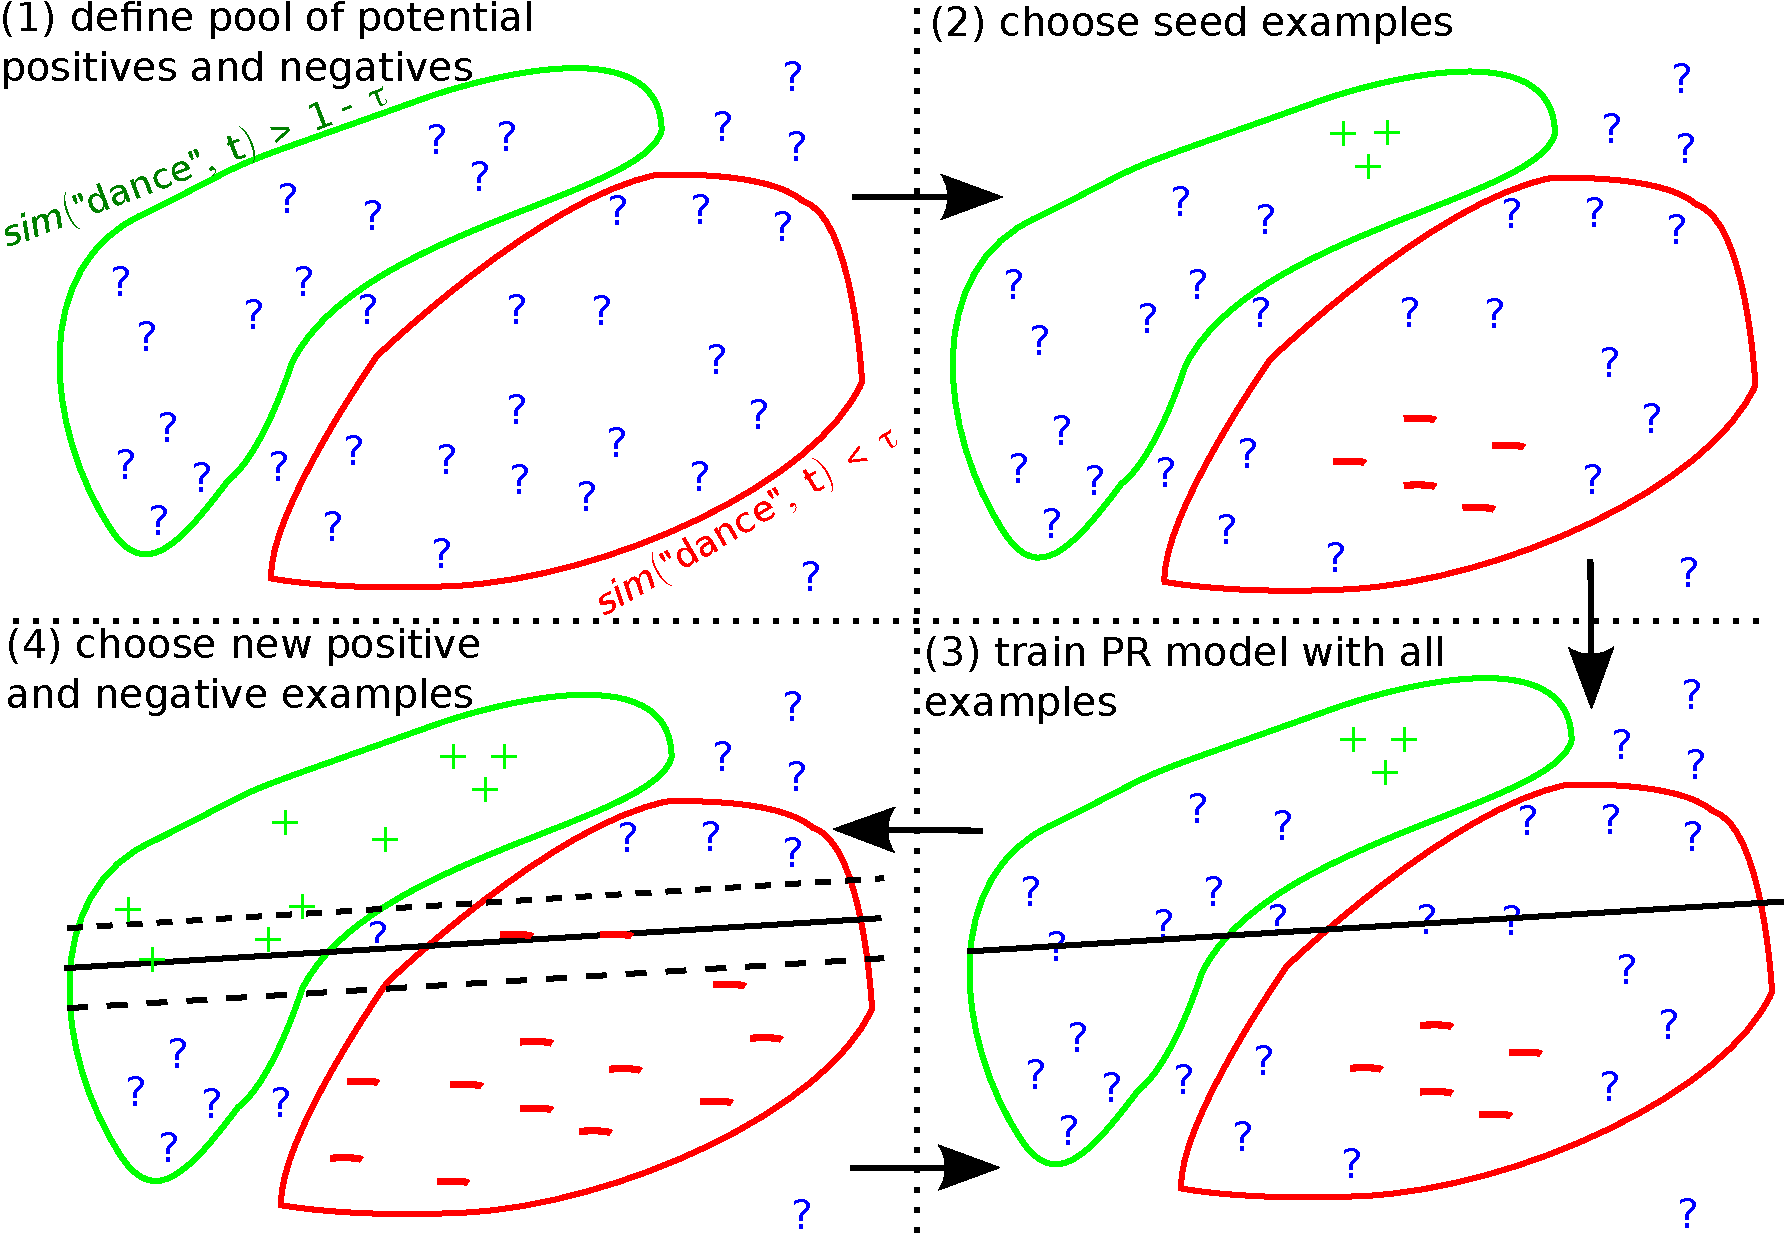
\includegraphics[scale = 0.27]{../images/system2b.pdf}
  \caption{An overview of our self-paced approach shown for one action or role. 
  The green and red boundaries indicate the positive and negative pool of samples chosen using the topic model SR.}
\label{fig:system2}
\end{figure}
% ---------------------------------------------------------------------------------

\vspace*{-4pt}

\subsection{Training event model}\label{sec:event_model}
We use the action and role detection probabilities to perform video event
classification. The expected number of tracklets corresponding to different
actions and roles are used as additional features along with the global video
features to train a linear ensemble SVM. We use the same set of global video
features from Sec.~\ref{sec:model_features}. Similar to \cite{Izadinia_ECCV12},
we first train separate event classifiers for each individual feature mentioned
in Sec.~\ref{sec:model_features} and finally treat the event classification
score from these classifiers as global video features. Since only a small set
of actions and roles are usually related to an event, we add an additional
$L_1$ regularization term for the action and role feature weights to encourage
only the relevant action and/or role probabilities to be selected.

\section{Experiments}

We test our event, action and role classification models on the TRECVID-MED11 event kit videos. 
The dataset contains videos belonging to $15$ complex event classes. 
Each video is accompanied by a synopsis describing the events in the video, 
and few of them mention the atomic actions and objects present in the video. 
We use the same training and testing splits as \cite{Izadinia_ECCV12}. 

\subsection{Implementation details}\label{sec:implementation_details}
We define \textit{crude} action labels $\tilde{y}_i$ and role labels
$\tilde{z}_i$ for each video $x_i$ based on simple text processing. We set
$\tilde{y}_i^a = 1$ if $t_i$ contains the action string $a$, $\tilde{y}_i^a =
-1$ if none of the natural language descriptions in the event class of $x_i$ contain
the action string $a$; otherwise, we set $\tilde{y}_i^a=0$. We define
$\tilde{z}_i^r \in \{-1,0,1\}$ similarly for the video $x_i$ and role $r$.
These crude labels are used to train baseline models not using the
complete video description as well as to initialize the self-paced scheme in
Sec.~\ref{sec:NLP}. The value of $\tau$ is set to consider the top $300$ and
$30$ videos closest to the action and role description respectively as
potential positives.

The CRF allows any arbitrary set of actions and roles. In our experiments, 
we train separate models for each action and role. 
While training an action model, we consider the relation of the action to all the roles including a null role. Thus, the action model makes a latent role assignment to a tracklet while identifying the action in the tracklet. Similarly, each role model performs latent action assignment to the tracklets while identifying presence of the role in the tracklet. In practice, this makes the learning more tractable and also performs better than training a single model considering all actions and roles together.

\subsection{Action and role classification} \label{sec:results_actionRoles}
A set of $62$ atomic events were used in \cite{Izadinia_ECCV12}. Some of these events were non-human actions like vehicle movement.
We select a subset of $46$ classes which involve one or more humans. We choose only these action classes which are directly mentioned 
at least once in the training data descriptions. We consider a set of $13$ roles appearing in different events, 
as listed in Tab. \ref{tab:results_role}. Each video in the test set is annotated with the actions and roles present in it for evaluation. 
  
The action and role classification performance is evaluated by computing the average precision 
on the testing data as shown in Tab. \ref{tab:results_action}, \ref{tab:results_role}. The expected number of tracklets performing an action in a videos is treated as the corresponding action score for the video. Similarly, the expected number of tracklets holding a role in a video provides the role score. 

Full model refers to the complete algorithm using video descriptions to train
PR models in a self-paced setting. The different baselines are explained below.
The first three baselines train only with crude labels $\langle \tilde{y}_i, \tilde{z}_i \rangle$.

\vspace*{-5pt}
\begin{itemize}
 \item global only: uses global video features to train a SVM.\vspace*{-7pt}
 \item simple PR: train action or role models without considering joint action-role relation in Eq.~\ref{eq:potential_tracklet}.\vspace*{-7pt}
 \item full PR: uses action-role relation in addition to tracklet features to train the PR model.\vspace*{-7pt}
 \item wiki SR \cite{Rohrbach_CVPR10}: trains full PR model by identifying positives and negative training examples based on the Wikipedia SR using a threshold as defined in Sec.~\ref{sec:implementation_details}.\vspace*{-7pt}
 \item topic SR: Our full model without outlier handling through self paced learning. \vspace*{-3pt} 
\end{itemize}

% ------------------------ Table of action results ----------------------
\setlength{\tabcolsep}{2.5pt}
\begin{table}
\begin{center}
\scalebox{0.9}
{\footnotesize
\begin{tabular}{|l|c|c|c|c|c|c|}
\hline
%{Action} & global & simple & full & wiki & topic & full \\
%& only & PR & PR & SR \cite{Rohrbach_CVPR10} & SR & model\\
{Action} & global only & simple PR & full PR & wiki SR & topic SR & full model \\
& & & & \cite{Rohrbach_CVPR10} & & \\
 %\cline{2-3}
 %& Total acc. & Total acc. \\
  \hline \hline
bending & 0.0604 & \textbf{0.0708} & 0.0689 & 0.0688 & 0.0586 & 0.0601 \\ 
blowing candles & 0.4616 & 0.4485 & 0.5088 & \textbf{0.5222} & 0.4934 & 0.5134 \\ 
carving & 0.2131 & 0.0229 & 0.0918 & 0.0794 & 0.0359 & \textbf{0.2348} \\ 
casting & 0.0046 & 0.0125 & 0.0118 & 0.0119 & \textbf{0.0141} & 0.0135 \\ 
clapping & 0.1433 & 0.1865 & \textbf{0.2720} & 0.2615 & 0.2236 & 0.2408 \\ 
cleaning & \textbf{0.0262} & 0.0047 & 0.0047 & 0.0048 & 0.0048 & 0.0240 \\ 
cutting & \textbf{0.1928} & 0.0794 & 0.0764 & 0.0776 & 0.0760 & 0.1906 \\ 
cutting cake & 0.0885 & 0.1361 & 0.1764 & \textbf{0.2803} & 0.1208 & 0.1764 \\ 
cutting fabric & \textbf{0.1896} & 0.0152 & 0.1541 & 0.1526 & 0.1557 & 0.1351 \\ 
dancing & 0.5941 & 0.5556 & 0.6189 & 0.6052 & \textbf{0.6357} & 0.6261 \\ 
drilling & 0.0570 & 0.0145 & 0.0142 & 0.0157 & 0.0661 & \textbf{0.0910} \\ 
drinking & 0.0258 & 0.0347 & 0.0445 & \textbf{0.0556} & 0.0421 & 0.0322 \\ 
eating & 0.0532 & 0.0522 & \textbf{0.0613} & 0.0558 & 0.0598 & 0.0569 \\ 
falling & 0.1081 & \textbf{0.1697} & 0.1523 & 0.1390 & 0.1513 & 0.1512 \\ 
flipping & 0.3995 & 0.4316 & \textbf{0.4554} & 0.2636 & 0.4364 & 0.4524 \\ 
hammering & 0.0794 & 0.0057 & 0.0056 & 0.0057 & \textbf{0.2743} & 0.2741 \\ 
jacking car & \textbf{0.0734} & 0.0185 & 0.0172 & 0.0164 & 0.0185 & 0.0373 \\ 
jumping & 0.5572 & 0.5184 & 0.5443 & \textbf{0.5734} & 0.5203 & 0.5586 \\ 
kissing & 0.1499 & 0.5232 & 0.4976 & \textbf{0.5318} & 0.4716 & 0.4976 \\ 
laughing & 0.0853 & 0.1508 & 0.1624 & 0.1605 & \textbf{0.1753} & 0.1611 \\ 
lighting candle & 0.0218 & 0.0437 & \textbf{0.0805} & 0.0772 & 0.0513 & 0.0631 \\ 
open door & 0.1276 & 0.0846 & 0.0692 & 0.0692 & \textbf{0.1285} & 0.0989 \\ 
petting & \textbf{0.0253} & 0.0103 & 0.0103 & 0.0103 & 0.0103 & 0.0115 \\ 
planing & 0.0525 & 0.0162 & 0.0140 & 0.0084 & 0.0449 & \textbf{0.0555} \\ 
play instrument & 0.1335 & 0.2424 & 0.2059 & \textbf{0.2705} & 0.2083 & 0.2059 \\ 
pointing & 0.0159 & 0.0437 & \textbf{0.0466} & 0.0398 & 0.0336 & 0.0238 \\ 
polishing & 0.0015 & 0.0015 & 0.0015 & 0.0015 & 0.0017 & \textbf{0.0025} \\ 
pouring & 0.0051 & 0.0061 & \textbf{0.0103} & 0.0038 & 0.0088 & 0.0026 \\ 
pushing & 0.2768 & \textbf{0.2871} & 0.1922 & 0.2865 & 0.1783 & 0.1824 \\ 
reeling & 0.4603 & 0.4675 & 0.4669 & \textbf{0.4973} & 0.4665 & 0.4788 \\ 
rolling & \textbf{0.0533} & 0.0074 & 0.0072 & 0.0065 & 0.0078 & 0.0091 \\ 
sawing & 0.0416 & 0.0305 & 0.0628 & 0.0667 & 0.0750 & \textbf{0.2390} \\ 
sewing & 0.3073 & \textbf{0.4089} & 0.2801 & 0.2839 & 0.2660 & 0.2588 \\ 
shake & 0.0067 & 0.0062 & 0.0062 & 0.0058 & 0.0064 & \textbf{0.0101} \\ 
singing & 0.0384 & 0.0900 & 0.0732 & 0.0721 & \textbf{0.0901} & 0.0742 \\ 
sliding & 0.0438 & \textbf{0.0811} & 0.0776 & 0.0750 & 0.0761 & 0.0806 \\ 
stir & 0.0398 & 0.2008 & 0.2037 & \textbf{0.2071} & 0.1975 & 0.1967 \\ 
surfing & 0.1039 & 0.1442 & 0.1494 & \textbf{0.1510} & 0.1302 & 0.1382 \\ 
turning wrench & \textbf{0.0788} & 0.0234 & 0.0233 & 0.0232 & 0.0232 & 0.0573 \\ 
using knife & 0.0015 & 0.0016 & 0.0017 & \textbf{0.0023} & 0.0016 & 0.0017 \\ 
using tire tube & \textbf{0.0675} & 0.0145 & 0.0141 & 0.0136 & 0.0138 & 0.0351 \\ 
walking & 0.1771 & 0.2562 & 0.2520 & 0.2110 & \textbf{0.2697} & 0.2557 \\ 
washing & \textbf{0.1329} & 0.0309 & 0.0307 & 0.0309 & 0.0307 & 0.0307 \\ 
waving & 0.0965 & 0.1302 & 0.1555 & 0.1413 & 0.1473 & \textbf{0.1700} \\ 
wiping & \textbf{0.0428} & 0.0253 & 0.0253 & 0.0253 & 0.0405 & 0.0369 \\ 
writing & 0.0400 & 0.1309 & 0.1080 & 0.1010 & 0.1413 & \textbf{0.1856} \\  
\hline \hline
mean & 0.1295 &   0.1356  &  0.1415 & 0.1427 & 0.1453 & \textbf{0.1616} \\
\hline
\end{tabular}
}
\end{center}
\caption{Action classification results. The highest score for a class is shown in bold font. The first three columns do not use the complete video descriptions, but train with labels $\langle \tilde{y}_i, \tilde{z}_i \rangle$.}
\label{tab:results_action}
\end{table}
\setlength{\tabcolsep}{1.4pt}
% ---------------------------------------------------------------------

% ------------------------ Table of role results ----------------------
\setlength{\tabcolsep}{2.5pt}
\begin{table}
\begin{center}
\scalebox{0.9}
{\footnotesize
\begin{tabular}{|l|c|c|c|c|c|c|}
\hline
%{Role} & global & simple & full & wiki & topic & full \\
%& only & PR & PR & SR \cite{Rohrbach_CVPR10} & SR & model\\
{Role} & global only & simple PR & full PR & wiki SR & topic SR & full model \\
& & & & \cite{Rohrbach_CVPR10} & & \\
  \hline \hline
bride & 0.7115 & 0.7946 & 0.7880 & 0.7873 & \textbf{0.8017} & 0.7877 \\ 
groom & 0.6751 & 0.7755 & 0.7805 & 0.7857 & 0.7901 & \textbf{0.7901} \\ 
priest & 0.2686 & 0.4263 & 0.4094 & \textbf{0.4468} & 0.4002 & 0.4058 \\ 
performer & 0.1499 & 0.1212 & 0.1708 & \textbf{0.1805} & 0.1722 & 0.1737 \\ 
musician & 0.0990 & \textbf{0.2933} & 0.2468 & 0.2506 & 0.2334 & 0.2643 \\ 
parent & 0.2084 & \textbf{0.2388} & 0.2123 & 0.2028 & 0.2014 & 0.2245 \\ 
birthday child & 0.7442 & 0.8350 & 0.8212 & 0.8086 & 0.8359 & \textbf{0.8359} \\ 
audience/guest & 0.3163 & 0.4260 & 0.3623 & 0.4263 & 0.3807 & \textbf{0.4429} \\ 
friends & 0.2849 & 0.5619 & \textbf{0.5671} & 0.4979 & 0.5591 & 0.5641 \\ 
fisherman & 0.2677 & 0.0238 & \textbf{0.2949} & 0.2617 & 0.2925 & 0.2873 \\ 
craftsman & \textbf{0.0957} & 0.0284 & 0.0281 & 0.0285 & 0.0282 & 0.0265 \\ 
mechanic & \textbf{0.0446} & 0.0268 & 0.0267 & 0.0262 & 0.0266 & 0.0264 \\ 
police/soldier & 0.2267 & 0.2346 & 0.2122 & \textbf{0.2398} & 0.2384 & 0.2303 \\ 
\hline \hline
mean & 0.3148  &  0.3682  &  0.3785  &  0.3802  &  0.3816 &  \textbf{0.3892}\\
\hline
\end{tabular}
}
\end{center}
\caption{Role classification results. The highest score for a class is shown in bold font. The first three columns do not use the complete video descriptions, but train with labels $\langle \tilde{y}_i, \tilde{z}_i \rangle$.}
\label{tab:results_role}
\end{table}
\setlength{\tabcolsep}{1.4pt}
% ---------------------------------------------------------------------------------

\vspace*{-3pt}

% -------- Action role matrix
\begin{figure}[ht!]
\centering
   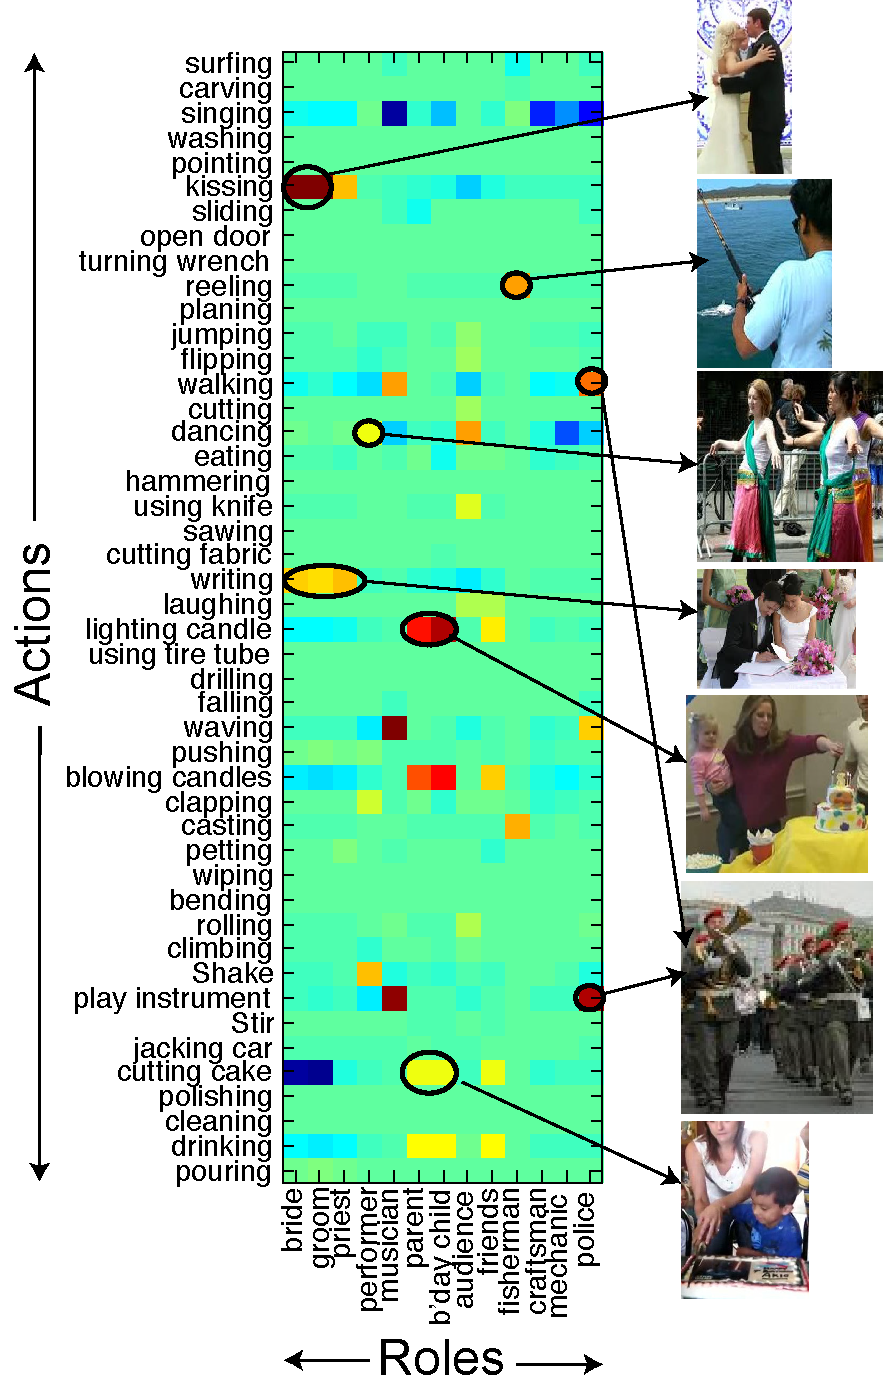
\includegraphics[scale = 0.48]{../images/ARmat2.pdf}
      \caption{The weights corresponding to different action-role relation $w_I(a,r)$ are shown. Sample frames depicting the action-role relations corresponding to some high weights are also shown.}
\label{fig:action_role_matrix}
\end{figure}
% ---------------------------------------------------------------------------------
\vspace*{-5pt}

Comparing the performance of global only and simple PR baselines in Tab.~\ref{tab:results_action}, \ref{tab:results_role}, we observe that identifying human tracklets in the videos improves the overall action as well as role classification. The effect is even more prominent for roles, since roles are governed by the humans holding the roles, whereas most actions like reeling, cutting, jacking car, turning wrench can be determined by object manipulations in the scene. We notice that actions like kissing, walking, playing instrument which can be determined by observing the complete or the upper human body, benefit more from the human tracklet representation compared to actions like cleaning, cutting, petting, turning wrench which are often shown as close-up shots of the hand. Similarly, human detectors fail to detect people when they are not upright, leading to a drop in performance.

From simple PR and full PR results in Tab.~\ref{tab:results_action},
\ref{tab:results_role}, we notice that jointly modeling the action-role
relations in the posterior regularized setup increases the performance for
action classes like kissing, writing, lighting candle, cutting cake and the
roles fisherman, birthday child, performer. In order to analyze the effect of
action-role relations, we visualize the joint action-role weights in
Fig.~\ref{fig:action_role_matrix}. As expected, we see strong correlation
between certain action and role classes (highlighted by ovals). These
correspondences result in an improved classification accuracy for the
respective classes. Sample frames pertaining to some high weights are shown
besides the matrix in Fig.~\ref{fig:action_role_matrix}. We further demonstrate
some qualitative results in Fig.~\ref{fig:actionRoleSamples}, where the highest
scoring tracklet in a video for a certain action is shown along with the
corresponding role assignment.

% -------- Sample results for youtube videos
\begin{figure}[ht]
\centering
   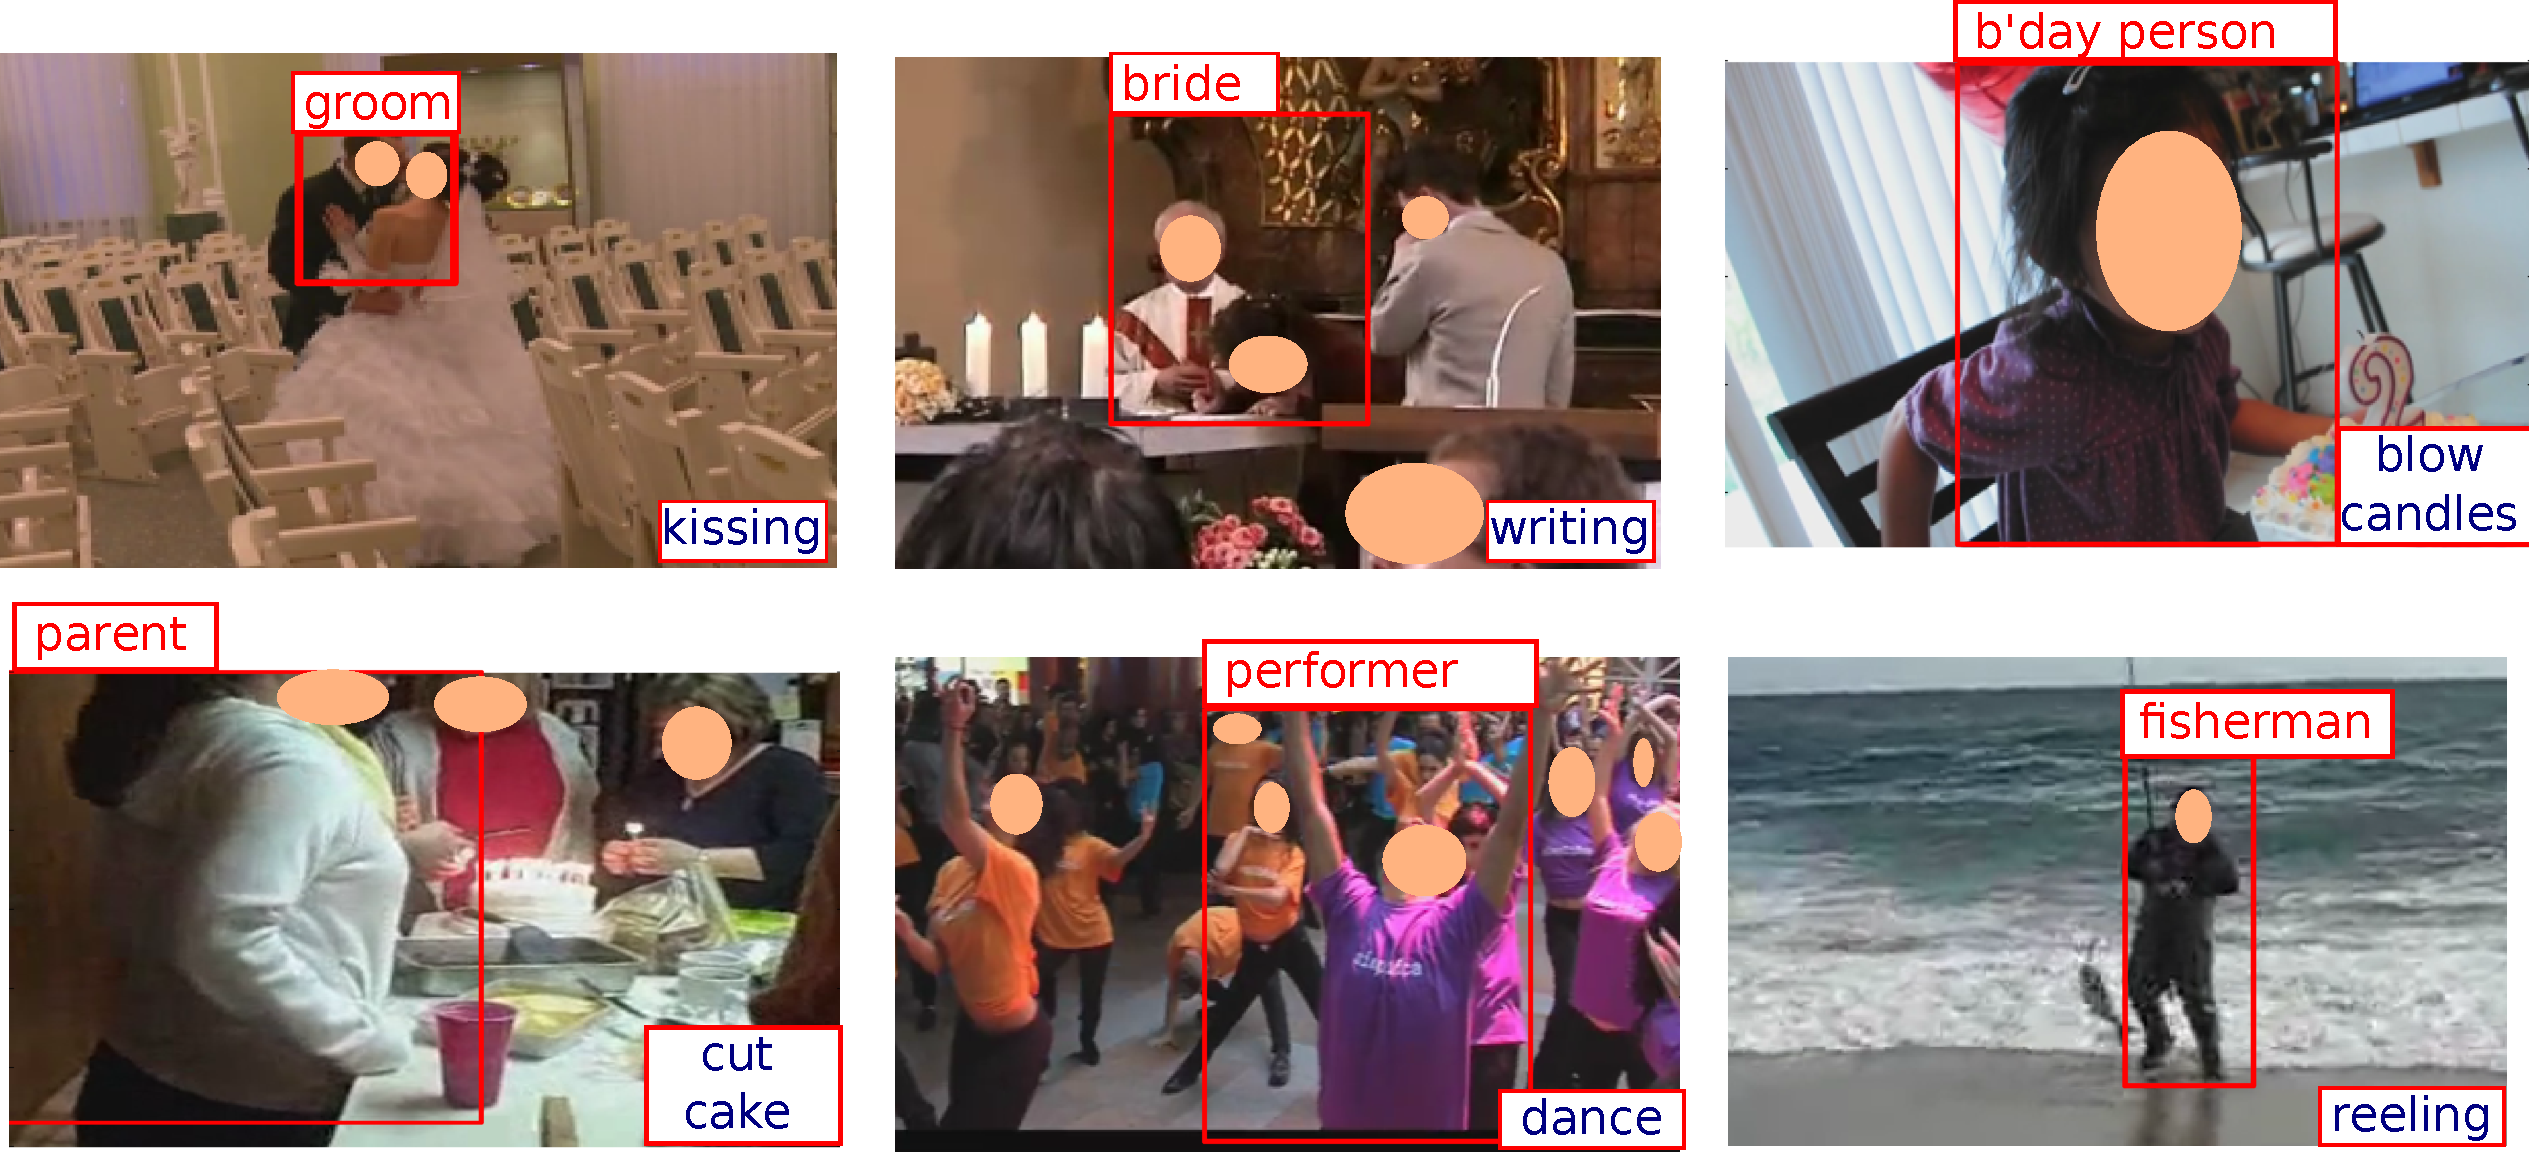
\includegraphics[scale = 0.2]{../images/actionRoleSamples.pdf}
      \caption{High scoring tracklets for few action models are shown for six test videos. The role assignments are also shown.}
\label{fig:actionRoleSamples}
\end{figure}
% ---------------------------------------------------------------------------------
\vspace*{-5pt}

The wiki SR and topic SR models trained by identifying positives and negatives based on a SR measure are seen to only marginally improve the performance. This can be accounted to the addition of false positive and negative training labels, demonstrating the difficulty in processing natural language descriptions. The results are seen to be worse in the case of Wikipedia based SR measure. %On the other hand, most human roles like ``bride, groom, priest'' do not have a varied representation in video descriptions. This is reflected in the similar performances of both the SR measures for role classification. 

To analyze the utility of our topic model, we run experiments 
where natural language descriptions are assumed to be present both
during training and testing. We train two separate PR models which use topic
model based textual features and Wikipedia SR based textual features
respectively as additional global features both during training and testing.
The mean AP of these models correspond to the green bars in
Fig.~\ref{fig:action_role_text}. For Wikipedia features, we concatenate the
Wikipedia SR measure of a description with each of the action and role strings
to form a feature. We treat $f_d$ as the topic model feature. The
considerable gain achieved by using topic model features during test time over
other methods justifies the use of topic model SR for the current task. The
lower performance of Wikipedia-based methods can be explained by the use of
generic corpus and lack of dimensionality reduction to consider concepts
specific to the task.

Further, note that in our adaptation of the self-paced approach, 
while natural language descriptions are not available during testing, 
we use features extracted from natural language descriptions in the initial iterations of training, 
and finally anneal their weights to zero. The effectiveness of our textual features as shown in Fig.~\ref{fig:action_role_text} allows us to 
handle outliers introduced by the SR measure.

% -------- Sample results for youtube videos
\addtolength{\subfigcapskip}{-0.1in}
\begin{figure}[ht!]
\centering
  \subfigure[actions]{
   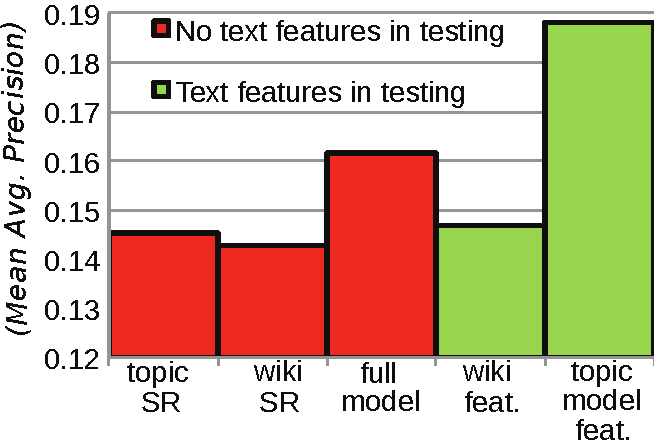
\includegraphics[scale = 0.35]{../images/actionPlot.pdf}
   }
   \subfigure[roles]{
   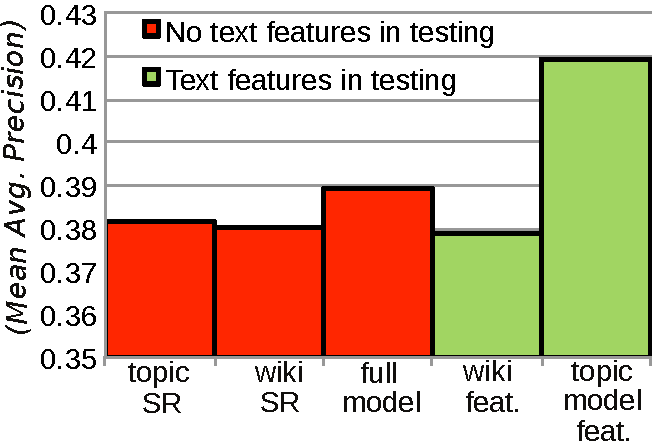
\includegraphics[scale = 0.35]{../images/rolePlot.pdf}
   }
      \caption{The green bars correspond to the setting where natural language descriptions are
      used at test time. The red bars
      are from Tab.~\ref{tab:results_action}, \ref{tab:results_role}.}
\label{fig:action_role_text}
\end{figure}
% ---------------------------------------------------------------------------------

From Tab.~\ref{tab:results_action}, \ref{tab:results_role},
we see that our full model, which handles outliers, is able to achieve
significant improvement over the other methods.
%baselines not using the complete video descriptions to train the model.
Our method is seen to be particularly
effective for action classes like
hammering, writing, planing, drilling, where the number of training video
descriptions directly containing the action string were below $10$. We show
sample videos which were added as positives by our full method in
Fig.~\ref{fig:added_positives}, along with the corresponding descriptions. We
notice the inclusion of videos whose descriptions do not contain the action
directly. 


% -------- Positives added by the method
\begin{figure*}[ht]
\centering
   \includegraphics[scale = 1]{../images/addedPositives.pdf}
      \caption{Videos with highest SR measure added as positives by our full method for different actions are shown. The last column shows wrong videos which are added by the method. The video descriptions are shown below it. Note that they do not contain the action string.}
\label{fig:added_positives}
\end{figure*}
% ---------------------------------------------------------------------------------

 

\subsection{Event classification}
We compare the event classification performance of our model from Sec.~\ref{sec:event_model} against baseline methods as well as state-of-the-art results from \cite{Izadinia_ECCV12} in Tab.~\ref{tab:results_event}. It is to be noted that unlike our method, \cite{Izadinia_ECCV12} used extensive spatio-temporal annotation to learn completely supervised atomic action classification models. The prediction probabilities from these models were finally used to perform event classification. We report two sets of results from \cite{Izadinia_ECCV12}, one using action classification scores in linear ensemble SVM and the other using them in a joint CRF model. In addition, we demonstrate results against the following baselines

\vspace*{-3pt}
\begin{itemize}
 \item global only: uses global video features only \vspace*{-9pt}
 \item global+actions : uses only action classification features in addition to global video features \vspace*{-9pt}
 \item global+roles: uses only role classification features in addition to global video features \vspace*{-5pt}
\end{itemize}
\vspace*{-3pt}

% ------------------------ Table of event classification results ----------------------
\setlength{\tabcolsep}{2.5pt}
\begin{table}
\begin{center}
\scalebox{0.9}
{\footnotesize
\begin{tabular}{|l|c|c|c|c|c|c|}
\hline
{Event} & global & \cite{Izadinia_ECCV12} {\color{red}*} & \cite{Izadinia_ECCV12} {\color{red}*} joint & global +  & global + & full \\
& only & SVM & CRF & action & roles & model \\
 %\cline{2-3}
 %& Total acc. & Total acc. \\
  \hline \hline
Boarding trick & \textbf{0.8766} & 0.7560 & 0.7570 & 0.8276 & 0.8625 & 0.8402 \\ 
Feeding animal & 0.4535 & \textbf{0.5820} & 0.5650 & 0.4490 & 0.3958 & 0.4595 \\ 
Landing fish & 0.6612 & \textbf{0.7410} & 0.7220 & 0.6612 & 0.6811 & 0.6593 \\ 
Wedding & 0.4729 & 0.6650 & 0.6750 & 0.5942 & 0.7555 & \textbf{0.7871} \\ 
Woodworking project & 0.2227 & 0.5760 & \textbf{0.6530} & 0.3697 & 0.2086 & 0.3568 \\ 
Birthday party & 0.9083 & 0.7090 & 0.7820 & \textbf{0.9207} & 0.9041 & 0.9008 \\ 
Changing tire & 0.5100 & 0.4650 & 0.4770 & \textbf{0.5200} & 0.4977 & 0.5012 \\ 
Flash mob & \textbf{0.9301} & 0.8590 & 0.9190 & 0.9273 & 0.9248 & 0.9240 \\ 
Vehicle unstuck & 0.6288 & 0.6610 & \textbf{0.6910} & 0.6212 & 0.5862 & 0.6173 \\ 
Grooming animal & 0.3881 & 0.4570 & 0.5100 & 0.3914 & 0.3927 & \textbf{0.5415} \\ 
Making sandwich & 0.5604 & 0.3560 & 0.4190 & \textbf{0.5739} & 0.5442 & 0.5704 \\ 
Parade & \textbf{0.7462} & 0.6570 & 0.7240 & 0.7283 & 0.6582 & 0.7335 \\ 
Parkour & 0.5426 & 0.5340 & \textbf{0.6640} & 0.6211 & 0.5681 & 0.6144 \\ 
Repairing appliance & 0.8025 & \textbf{0.8080} & 0.7820 & 0.7989 & 0.7692 & 0.7840 \\ 
Sewing project & 0.6579 & 0.5690 & 0.5750 & 0.6563 & 0.6286 & \textbf{0.6688} \\ 
\hline \hline
mean & 0.6241 & 0.6263 & 0.6610 & 0.6441 & 0.6252 & \textbf{0.6639} \\
\hline
\end{tabular}
}
\end{center}
\caption{Event classification results. The highest score for a class is shown in bold font. {\color{red}*} Unlike our method, \cite{Izadinia_ECCV12} uses extensive ground truth spatio-temporal annotations for training separate action classifiers to aid event classification.}
\label{tab:results_event}
\end{table}
\setlength{\tabcolsep}{1.4pt}
% ---------------------------------------------------------------------------------

From Tab.~\ref{tab:results_event}, we observe that our methods using either the
action or role features outperform an SVM trained only with global video
features. Our full model using both action and role scores achieves the maximum
mean AP. Thus, our action and role models trained only with natural language
descriptions matches state-of-the-art methods from \cite{Izadinia_ECCV12},
which uses ground truth spatio-temporal action annotations for training. This
confirms the utility of the our action and role models learned with very weak
supervision.

\section{Conclusion}
We have presented a method to learn atomic action and role models based on easily available natural language video descriptions. We proposed a language topic-model based semantic relatedness measure to identify positive and negative training examples. These labels were used to train a CRF model with posterior regularization, while making latent action and role assignments to human tracklets. Outliers introduced by the SR measure were handled through a self-paced scheme. The action and role models were used to achieve state-of-the-art event classification performance on the TRECVID-MED11 event kits. We demonstrated the efficacy of the topic model based SR measure in identifying training labels as well as the gain due to the posterior regularized method in a weakly supervised setting without temporal annotations. In future work, we wish to ground action-object relations in complex event videos based on natural language descriptions and simultaneously learn these relation from both textual and visual data.

\section*{Acknowledgements}
We thank O. Russakovsky, K. Tang and B. Yao for helpful comments. This research is partially supported by Intel, 
the NFS grant $IIS-1115493$ and DARPA-Mind's Eye grant.


{\small
\bibliographystyle{ieee}
\bibliography{TextActionRoles}
}

\end{document}
